\let\negmedspace\undefined
\let\negthickspace\undefined
\documentclass[journal]{IEEEtran}
\usepackage[a5paper, margin=10mm, onecolumn]{geometry}
%\usepackage{lmodern} 
\usepackage{tfrupee} 

\setlength{\headheight}{1cm} 
\setlength{\headsep}{0mm}     

\usepackage{gvv-book}
\usepackage{gvv}
\usepackage{cite}
\usepackage{amsmath,amssymb,amsfonts,amsthm}
\usepackage{algorithmic}
\usepackage{graphicx}
\usepackage{textcomp}
\usepackage{xcolor}
\usepackage{txfonts}
\usepackage{listings}
\usepackage{enumitem}
\usepackage{mathtools}
\usepackage{gensymb}
\usepackage{comment}
\usepackage[breaklinks=true]{hyperref}
\usepackage{tkz-euclide} 
\usepackage{listings}                                        
\def\inputGnumericTable{}                                 
\usepackage[latin1]{inputenc}                                
\usepackage{color}                                            
\usepackage{array}                                            
\usepackage{longtable}                                       
\usepackage{calc}                                             
\usepackage{multirow}                                         
\usepackage{hhline}                                           
\usepackage{ifthen}                                           
\usepackage{lscape}

\begin{document}

\bibliographystyle{IEEEtran}
\vspace{3cm}

\title{4.7.64}
\author{AI25BTECH11003 - Bhavesh Gaikwad}
{\let\newpage\relax\maketitle}

\renewcommand{\thefigure}{\theenumi}
\renewcommand{\thetable}{\theenumi}
\setlength{\intextsep}{10pt} 


\numberwithin{equation}{enumi}
\numberwithin{figure}{enumi}
\renewcommand{\thetable}{\theenumi}


\textbf{Question}: Find the distance between the point $\vec{P}$(6, 5, 9) and the plane determined by the points $\vec{A}$(3, -1, 2), $\vec{B}$(5, 2, 4) and $\vec{C}$(-1, -1, 6). \\

\textbf{Solution:}\\
Given:
\begin{equation}
\vec{P} = \myvec{6 \\ 5 \\ 9}, \, \vec{A} = \myvec{3 \\ -1 \\ 2}, \, \vec{B} = \myvec{5 \\ 2 \\ 4}, \, \vec{C} = \myvec{-1 \\ -1 \\ 6}
\end{equation}\\

Let $\vec{n}$ be the perpendicular vector to plane.

\begin{equation}
    \vec{n} = \vec{(B-A)} \times \vec{(C-A)} = \myvec{|\vec{A_{23}} & \vec{B_{23}}| \\ |\vec{A_{31}} & \vec{B_{31}}| \\ |\vec{A_{12}} & \vec{B_{12}}|} = \myvec{12 \\ -16 \\ 12}
\end{equation}\\

\begin{center}
    OR
\end{center}

\begin{equation}
\vec{n} = \myvec{3 \\ -4 \\ 3}
\end{equation}\\

if $\vec{n} = \myvec{\alpha \\ \beta \\ \gamma}$ then the equation of the plane would be
\begin{equation}
    \alpha(x) + \beta(y) + \gamma(z) = k \text{, Where k is a constant}
\end{equation}\\

From Equation 0.3 and 0.4, 
\begin{equation}
    \alpha = 3, \, \beta = -4, \, \gamma = 3
\end{equation}

\begin{equation}
\therefore
\text{ The equation of the plane will be } 3x-4y+3z = k.
\end{equation}


Putting Coordinates of $\vec{A}$ in equation 0.6 to get k,
\begin{equation}
    k=3(3) - 4(-1) + 3(2) \quad \Rightarrow k= 19
\end{equation}

\begin{equation}
\therefore \, 3x-4y+3z=19
\end{equation}

Let $\vec{L}$ be the line perpendicular to plane and passing through $\vec{P}$.\\
Let $\vec{Q}$ be a position vector of a point on the plane and the line $\vec{L}$

\begin{equation}
\text{From Equation 0.3, } \Rightarrow 
\vec{L} = \vec{P} + t\vec{n}
\quad \Rightarrow \vec{L} = \myvec{6 \\ 5 \\ 9} + t\myvec{3 \\ -4 \\ 3}
\end{equation}


Therefore from Equation 0.9,
$\vec{Q} = \myvec{6+3t \\ 5-4t \\ 9+3t}$

Putting co-ordinates of $\vec{Q}$ in equation of plane (from equation 0.8).

\begin{equation}
    3(6+3t) - 4(5-4t) + 3(9+3t) = 19 \quad \Rightarrow t=-\dfrac{3}{17}  
\end{equation}

\begin{equation}
    \therefore \, \vec{Q}=\myvec{93/17 \\ 97/17 \\ 144/17}
\end{equation}\\


The Distance between the plane and $\vec{P}$ is $\norm{\vec{P} - \vec{Q}}$
\begin{equation}
\norm{\vec{P} - \vec{Q}}= \norm{\myvec{9/17 \\ -12/17 \\ 9/17}} = \dfrac{3\sqrt{34}}{17}
\end{equation}\\\\


\begin{align}
    \boxed{\text{The Distance between the Plane and } \vec{P} \, is \, \dfrac{3\sqrt{34}}{17} \, units.}
\end{align}


\begin{figure}[htbp]
    \centering
    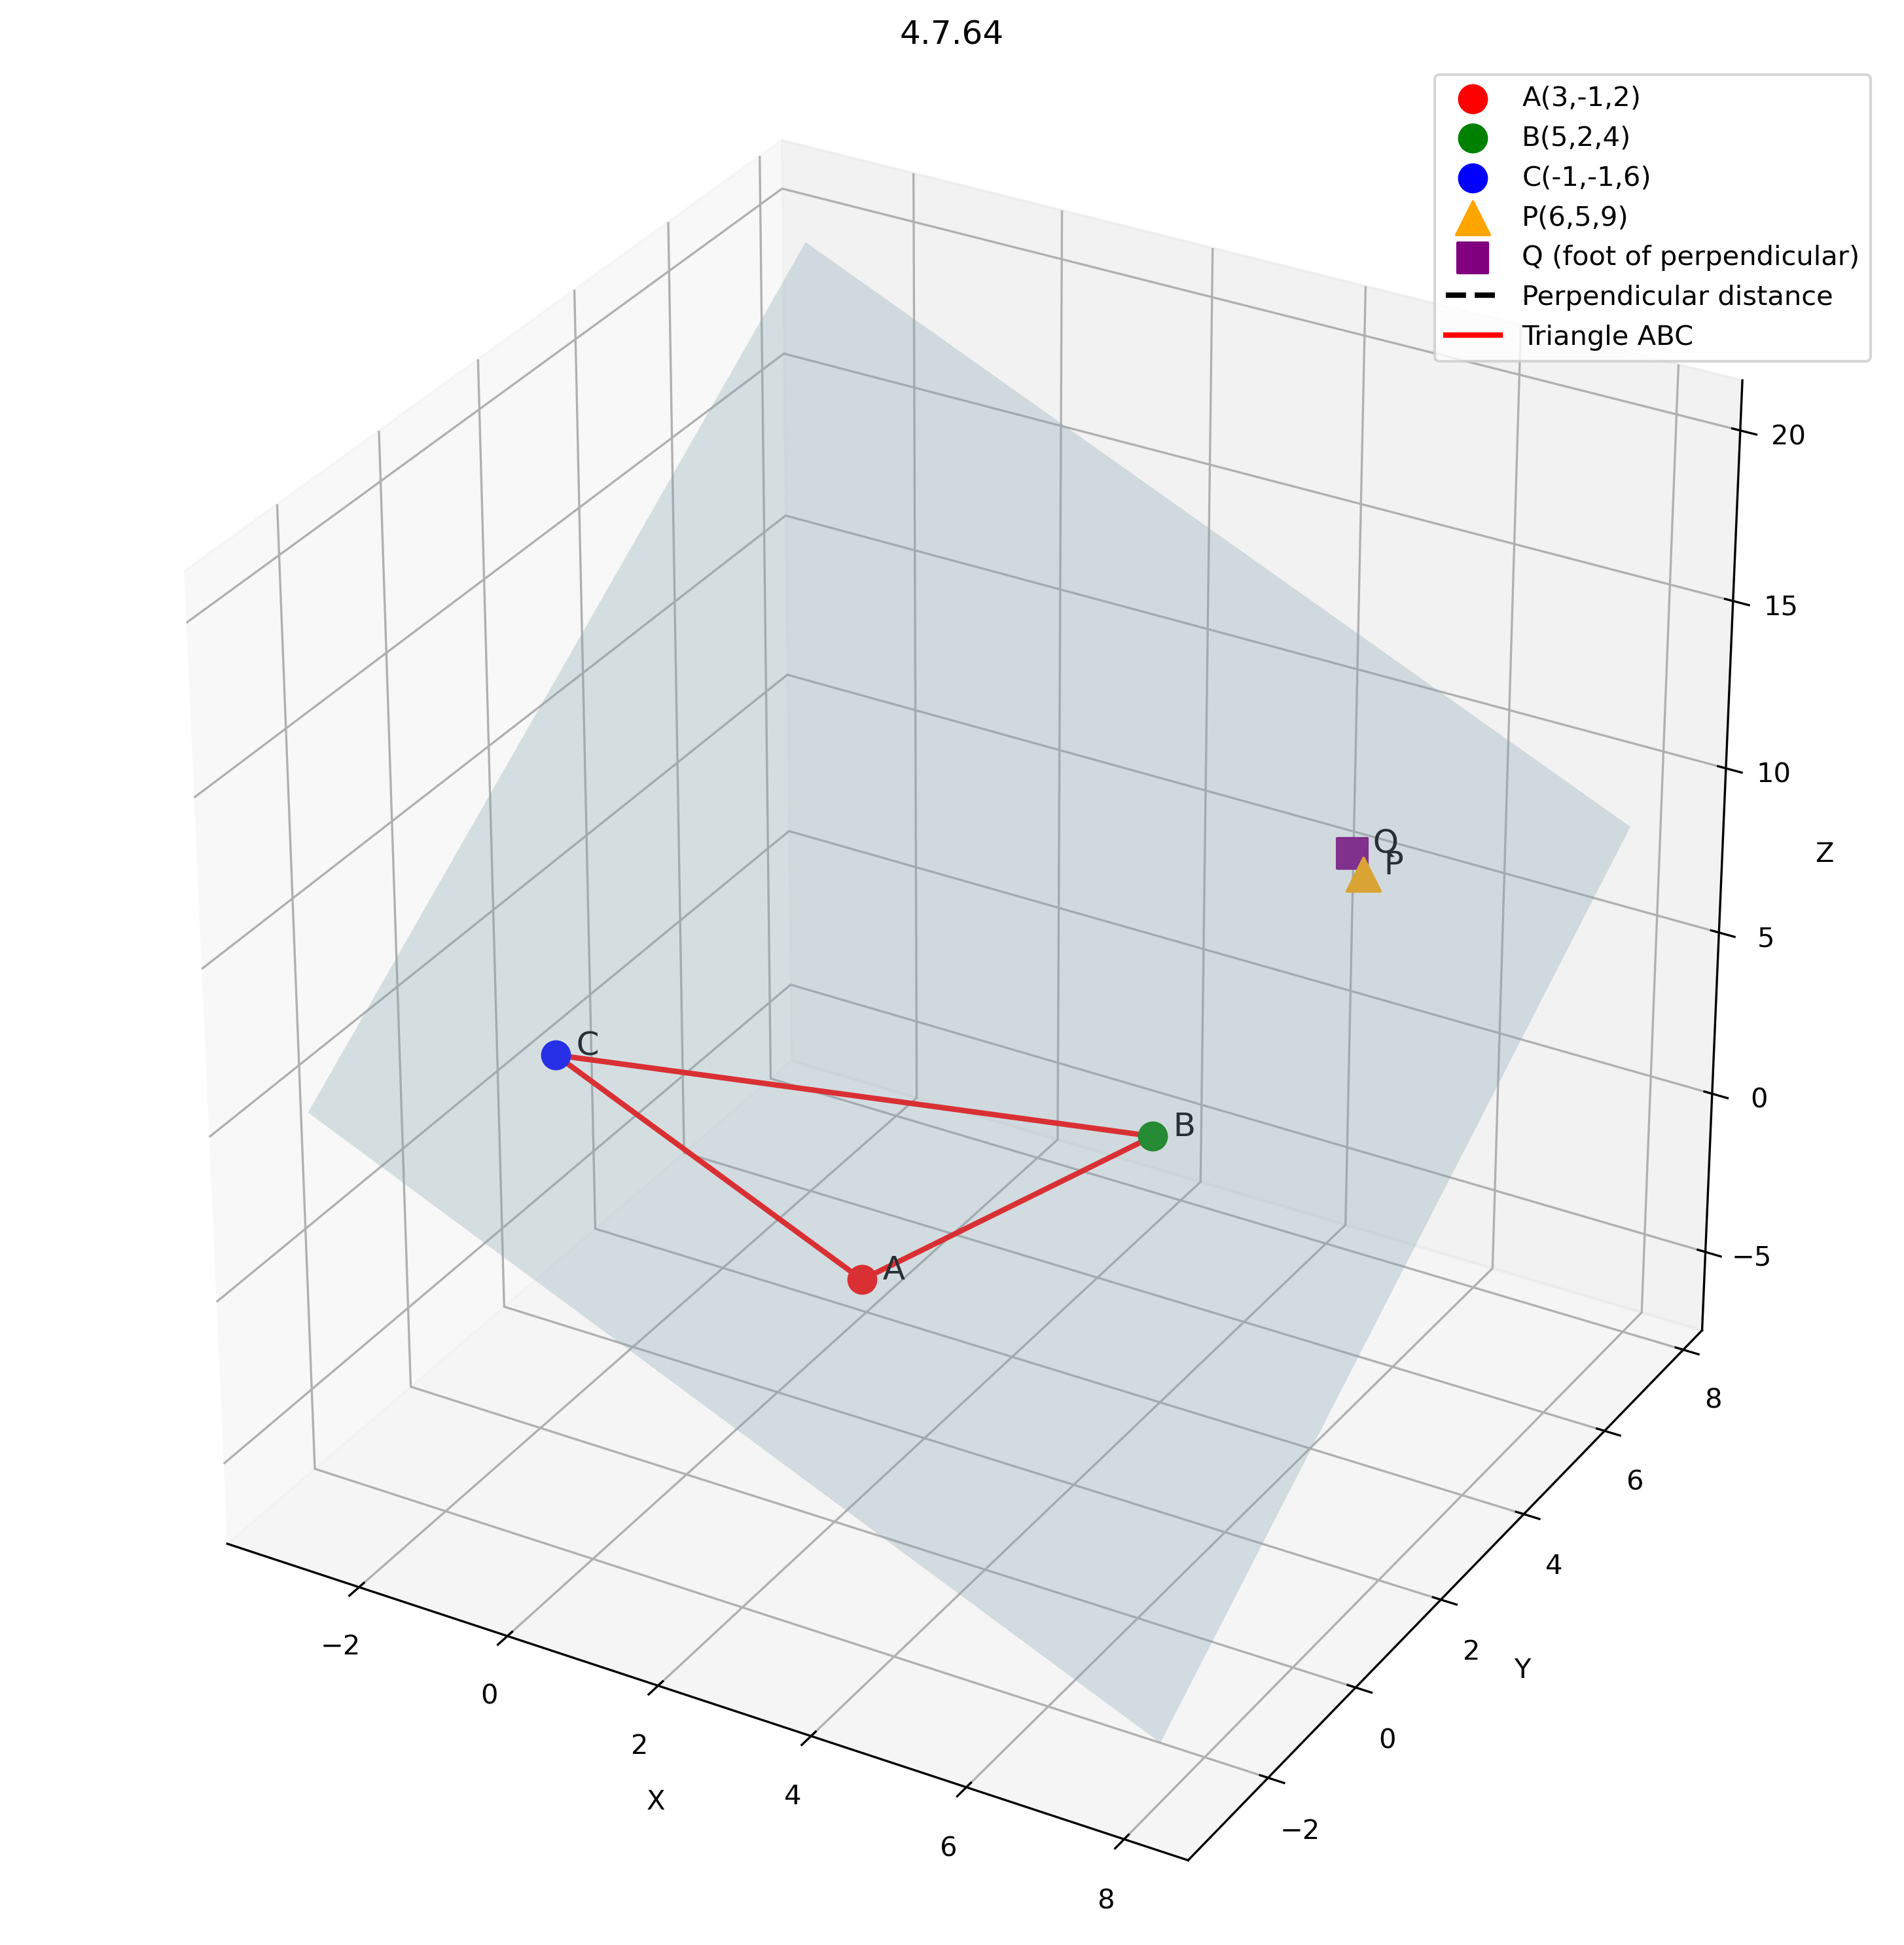
\includegraphics[width=\columnwidth]{figs/fig1.png}
    \caption{Plane}
    \label{fig:fig/fig1.png}
\end{figure}
\end{document}  
